\section{Evaluation Metrics}\label{sec:evaluation_metrics}
To justify the improvements stated in the hypothesis, a detailed evaluation based on the metrics described below was performed. 

We used two approaches to measure the performance of the crowd. The first one requires some reference data which is compared against empirical data. This approach, originating from Information Retrieval~(IR), is called the \textbf{Golden~Standard~Approach}~\cite{brank2005}. To quantify the improvements/degradations, several metrics exist. On a binary classification scheme, as illustrated in \hyperref[fig:binary_classification_metrics]{Figure~\ref*{fig:binary_classification_metrics}}, these metrics are defined as fractions of \emph{True~Positives~(TP)}, \emph{True~Negatives~(TN)}, \emph{False~Positives~(FP)} and \emph{False~Negatives~(FN)}.
\begin{figure}
	 \centering
	 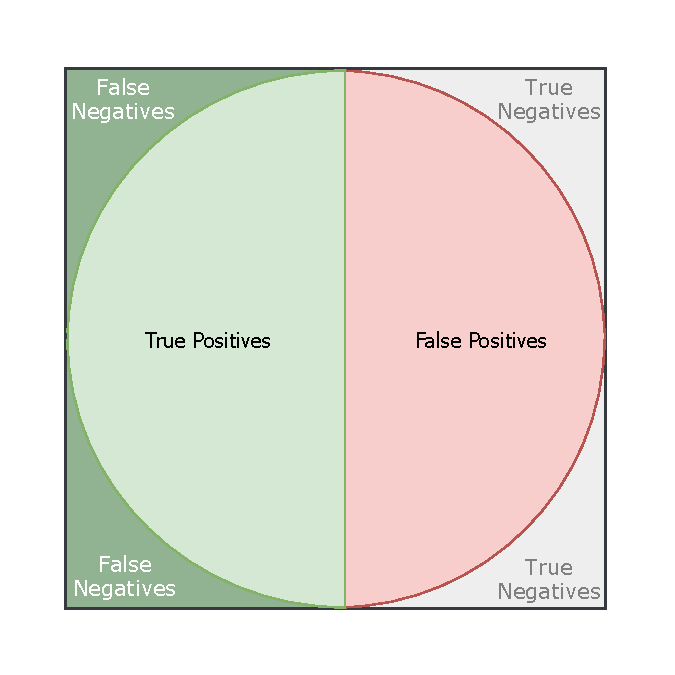
\includegraphics[width=0.5\textwidth]{drawio/Binary_Classification_Scheme}
	 \caption{Binary classification scheme for evaluation metrics of crowdsourcing tasks}\label{fig:binary_classification_metrics}
\end{figure}
In crowdsourcing contexts this means that yes-questions are either correctly~(TP) or incorrectly~(FN) answered and no-questions are either correctly answered~(TN) or incorrectly~(FP).

\paragraph{Precision} Precision is interpreted as the ratio of correctly answered yes-questions over the total number of answered yes-questions:
\[ Precision = \frac{TP}{TP + FP} \]
For concept relevance, values of Precision close to $1.0$ show that the crowd correctly rejects irrelevant concepts but maybe fails at accepting relevant ones. 
\paragraph{Recall} Recall is interpreted as the ratio of correctly answered yes-questions over the total number of available yes-questions:
\[ Recall = \frac{TP}{TP + FN} \]
For concept relevance, values of Recall close to $1.0$ show that the crowd correctly predicts relevant concepts but maybe fails at rejecting irrelevant ones. 

\paragraph{F-Measure} Unfortunately, exclusively relying on either of the above metrics has some drawbacks. For example, the crowd may correctly identify relevant concepts but fails at rejecting irrelevant ones~(high~Recall) or, on the other hand, irrelevant concepts may be correctly rejected whereas not all relevant ones may be detected~(high~Precision). 

The F-Measure compensates these flaws by combining Precision and Recall rates. The traditional F-Measure or balanced F-Score is calculated as the harmonic mean of Precision~(P) and Recall~(R):
\[ \mathit{F \mhyphen Measure} = 2 \cdot \frac{P \cdot R}{P + R} \]
In some situations researchers have criticised this metric that it may be biased~\cite{powers2011}. For this reason, there exists a modified version of the general F-Measure which takes an additional parameter $\beta$ into account:
\[ F_\beta = (1 + \beta^2) \cdot \frac{P \cdot R}{\beta^2 \cdot P + R} \]
Depending on the importance of Precision or Recall, $\beta$ can be set to a higher value~(e.g.~$F_2$), which weights Recall higher, or to a lower value~(e.g.~$F_{0.5}$), which puts more emphasis on Precision. Mostly, the generic F-Measure, also known as $F_1$ measure, is sufficient though, in which $\beta$ is set to $1$ to weight Precision and Recall evenly. 

The other approach in measuring the crowd's performance does not rely on reference values, instead, the metric reflects the agreement ratio among crowd workers. Therefore, the agreement ratio or \textbf{Inter-rater Agreement} measures, to what extend judges reached consensus. For binary tasks~(e.g. concept relevance checks), all possible outcomes are based on a table of 2x2~frequencies, as shown in \hyperref[fig:2x2_inter_rater_table]{Figure~\ref*{fig:2x2_inter_rater_table}}. In terms of evaluating concept relevance, this means that the crowd either agrees or disagrees whether a concept is relevant or not. 
\begin{figure}
	 \centering
	 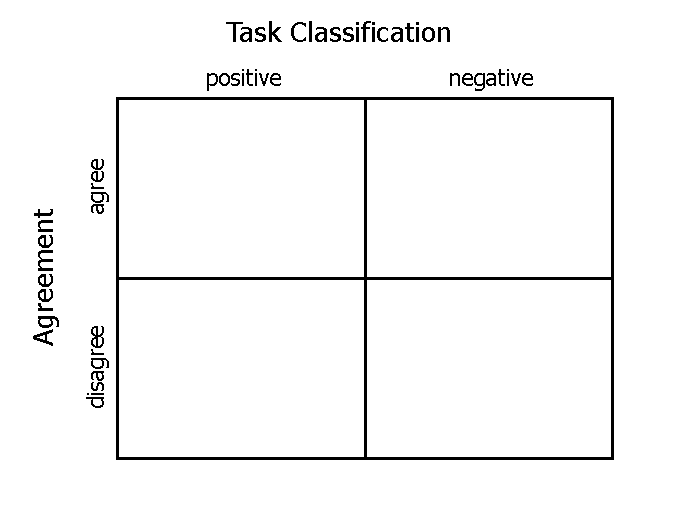
\includegraphics[width=0.5\textwidth]{drawio/Inter_Rater_Outcome_Table}
	 \caption{2x2 outcome table on Inter-rater Agreement for binary tasks}\label{fig:2x2_inter_rater_table}
\end{figure}

Several metrics exist to measure inter-rater reliability~\cite{zhao2013}. They primarily differ in to what extent judgements made by chance are taken into account. In our evaluation though, the following metric is used:
\paragraph{Percentage Agreement}
This is the simplest and most commonly used metric, which is calculated by dividing the number of agreeing raters~($A$) by the total rater count~($N$).
\[ Agreement = \frac{A}{N} \]
Despite its intuitive appeal, it has been criticised, that it does not take the agreements made by chance into account~\cite{hunt1986}. On the other hand, calculation of chance-adjusted metrics is more complex and have the potential to over- or undervalue the corrections for chance.  
Moreover, reliability is assumed to be very high because crowdsourcing settings were adjusted to sort out random answers. A more detailed discussion on this topic is given, when the evaluation setup is described.  
